

\subsection{Nghiên cứu so sánh và lựa chọn Game Engine}
Game engine là một phần mềm chuyên dụng được sử dụng để thiết kế và phát triển trò chơi điện tử. Có thể hiểu đơn giản, game engine đóng vai trò là một phần mềm trung gian, kết nối và quản lý sự tương tác giữa nhiều thành phần trong cùng một hệ thống trò chơi. Các chức năng cốt lõi của game engine chủ yếu liên quan đến việc làm việc trực tiếp với phần cứng, bao gồm: công cụ dựng hình đồ họa hai chiều và ba chiều, hệ thống vật lý dùng để phát hiện và xử lý va chạm, xử lý âm thanh, quản lý hình ảnh động.\\

Ngoài các chức năng cơ bản, nhiều game engine hiện nay còn tích hợp các gói mở rộng nhằm hỗ trợ những tính năng nâng cao như kết nối mạng, xử lý luồng dữ liệu, tối ưu hóa quá trình kết xuất hình ảnh và hiệu năng của trò chơi. Nhờ có game engine, quá trình phát triển trò chơi điện tử được rút ngắn đáng kể, giúp lập trình viên tiết kiệm thời gian và công sức thông qua việc tái sử dụng và mở rộng các thành phần có sẵn để tạo ra nhiều sản phẩm game khác nhau.\\

Hiện nay, trên thị trường có rất nhiều game engine với những ưu điểm và hạn chế riêng, phù hợp với từng thể loại trò chơi và mục đích phát triển khác nhau. Một số game engine phổ biến sẽ được trình bày ở các mục tiếp theo.

\subsubsection{Unity}

\begin{figure} [H]
    \centering
    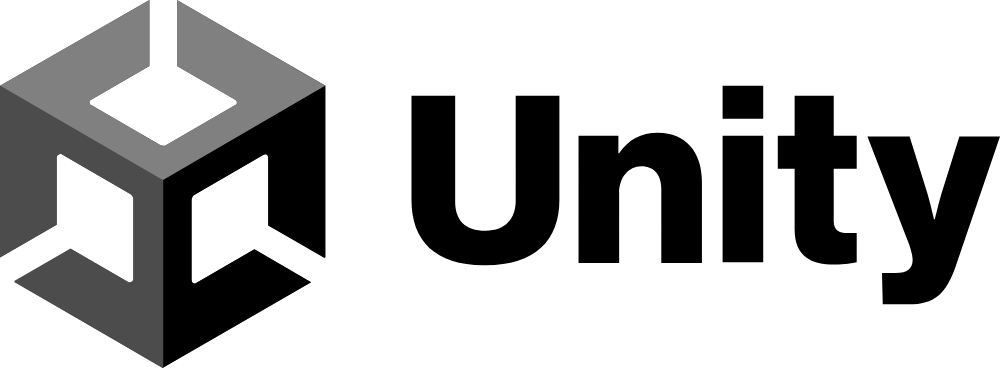
\includegraphics[width=0.4\linewidth]{3.Nghiên cứu//Images/Unity.png}
    % \caption{Unity}
    \label{fig:placeholder}
\end{figure}
Unity là một game engine được phát hành lần đầu vào năm 2005 và nhanh chóng trở thành một trong những nền tảng phát triển trò chơi phổ biến nhất hiện nay. Unity được nhiều nhà phát triển lựa chọn nhờ tính linh hoạt, dễ sử dụng và khả năng hỗ trợ xây dựng trò chơi đa nền tảng như Windows, Linux, macOS, thiết bị di động (Android, iOS) và trình duyệt web. Game engine này đặc biệt phổ biến trong lĩnh vực phát triển game di động và các trò chơi độc lập (indie).\\

Unity hỗ trợ phát triển cả trò chơi hai chiều (2D) và ba chiều (3D), cho phép mô phỏng các tương tác và hiệu ứng trong môi trường ảo một cách trực quan. Ngôn ngữ lập trình chính được sử dụng trong Unity là C\#, giúp lập trình viên dễ dàng tiếp cận và phát triển các chức năng cho trò chơi. Bên cạnh đó, Unity còn hỗ trợ các pipeline kết xuất hình ảnh hiện đại như HDRP (High Definition Render Pipeline) và URP (Universal Render Pipeline), giúp nâng cao chất lượng đồ họa và tối ưu hiệu năng.\\

Ngoài các công cụ phát triển cốt lõi, Unity còn cung cấp kho tài nguyên phong phú thông qua Unity Asset Store, bao gồm mô hình 3D, âm thanh, plugin và các công cụ hỗ trợ phát triển game. Đồng thời, Unity sở hữu một cộng đồng phát triển lớn và năng động, sẵn sàng hỗ trợ và giải đáp các thắc mắc cho người mới. Nhờ những ưu điểm trên, Unity là một lựa chọn phù hợp cho việc phát triển đồ án lập trình game của nhóm.


\subsubsection{Unreal Engine}

\begin{figure} [H]
    \centering
    
\includegraphics[width=0.3\linewidth]{3.Nghiên cứu//Images/Unreal.png}
    % \caption{Unreal Engine}
    \label{fig:placeholder}
\end{figure}
Unreal Engine là một game engine mạnh mẽ do Epic Games phát triển, được phát hành lần đầu vào năm 1998 và hiện nay đã trở thành một trong những công cụ phổ biến nhất trong lĩnh vực phát triển game 3D. Unreal Engine được sử dụng rộng rãi để phát triển các trò chơi có đồ họa chất lượng cao trên nhiều nền tảng như Windows, macOS, Linux, console và thiết bị di động.\\

Unreal Engine hỗ trợ lập trình bằng ngôn ngữ C++ và hệ thống lập trình trực quan Blueprint, giúp cả lập trình viên chuyên nghiệp lẫn người mới đều có thể tiếp cận và phát triển trò chơi. Engine này nổi bật với khả năng kết xuất hình ảnh chân thực, hệ thống ánh sáng tiên tiến, vật lý mạnh mẽ và các công cụ hỗ trợ trí tuệ nhân tạo cho nhân vật trong game.\\

Ngoài ra, Unreal Engine còn cung cấp nhiều công cụ hỗ trợ phát triển như hệ thống vật lý, âm thanh, mạng và tối ưu hiệu năng. Cùng với cộng đồng người dùng lớn và kho tài nguyên phong phú, Unreal Engine là lựa chọn phù hợp cho các dự án game quy mô lớn và các trò chơi đòi hỏi chất lượng đồ họa cao.


\subsubsection{Godot}

\begin{figure} [H]
    \centering
    
\includegraphics[width=0.4\linewidth]{Godot.png}
    % \caption{Godot Engine}
    \label{fig:placeholder}
\end{figure}
Godot là một game engine mã nguồn mở được phát triển nhằm phục vụ cho việc xây dựng các trò chơi 2D và 3D. Godot nổi bật với ưu điểm miễn phí hoàn toàn, không yêu cầu trả phí bản quyền và cho phép người dùng toàn quyền chỉnh sửa mã nguồn theo nhu cầu. Nhờ đó, Godot được sử dụng rộng rãi trong cộng đồng lập trình game độc lập (indie) và giáo dục.\\

Godot hỗ trợ đa nền tảng như Windows, Linux, macOS, Android, iOS và trình duyệt web. Engine này sử dụng các ngôn ngữ lập trình như GDScript (ngôn ngữ riêng của Godot có cú pháp tương tự Python), C\#, và C++. Hệ thống scene và node của Godot giúp việc tổ chức đối tượng trong game trở nên rõ ràng, linh hoạt và dễ quản lý.\\

Ngoài ra, Godot còn tích hợp sẵn các hệ thống vật lý, âm thanh, xử lý va chạm, hoạt ảnh và trí tuệ nhân tạo. Với dung lượng nhẹ, giao diện thân thiện, cộng đồng phát triển ngày càng lớn và tài liệu hướng dẫn phong phú, Godot là một lựa chọn phù hợp cho các dự án game nhỏ, game học tập và đồ án lập trình game.

\subsubsection{So sánh các game engine}
Mỗi phần mềm Game engine đều có các đặc điểm nổi trội riêng, Do đó để phân tích rõ hơn việc lựa chọn giữa các Game engine để thực hiện dự án, dưới đây là bảng so sánh điểm mạnh và điểm yếu giữa các phần mềm Game engine:

\begin{table}[H]
\centering
\begin{tabular}{|p{2cm}|p{4cm}|p{4cm}|p{4cm}|}
\hline
\textbf{Tiêu chí} & \textbf{Unity} & \textbf{Unreal Engine} & \textbf{Godot} \\
\hline
\textbf{Ngôn ngữ} 
& C\#: Dễ học, phổ biến 
& C++ / Blueprint: Mạnh, khó 
& GDScript: Giống Python, dễ \\
\hline
\textbf{Đồ họa} 
& Tốt (URP, HDRP) 
& Rất cao (Nanite, Lumen) 
& Khá, nhẹ \\
\hline
\textbf{2D/3D} 
& Mạnh cả 2D và 3D 
& Mạnh 3D 
& Mạnh 2D, 3D cơ bản \\
\hline
\textbf{Hiệu năng} 
& Tốt, ổn định 
& Rất cao 
& Nhẹ, đủ dùng \\
\hline
\textbf{Cộng đồng} 
& Rất lớn 
& Lớn 
& Đang phát triển \\
\hline
\textbf{Phần cứng} 
& Trung bình 
& Cao 
& Thấp \\
\hline
\textbf{Networking} 
& Mạnh (Netcode, Photon) 
& Tích hợp tốt 
& Cơ bản \\
\hline
\textbf{Chi phí} 
& Miễn phí cơ bản 
& Có phí theo điều kiện 
& Miễn phí 100\% \\
\hline
\textbf{Phù hợp} 
& Mobile, Indie, AR/VR 
& AAA, đồ họa cao 
& Học tập, Indie nhỏ \\
\hline
\end{tabular}
\caption{So sánh ngắn gọn Unity, Unreal Engine và Godot}
\end{table}


\textbf{Kết luận:} Nhóm chọn \textbf{Unity} vì sự cân bằng giữa hiệu năng và tính dễ sử dụng của ngôn ngữ C\#, đồng thời hệ sinh thái hỗ trợ Multiplayer của Unity rất phong phú phù hợp cho quy mô nhóm sinh viên.